\documentclass[]{article}
\usepackage{setspace}
\usepackage{graphicx}
\usepackage{hyperref}
\usepackage[font=small,labelfont=bf]{caption}
\usepackage{palatino}
\usepackage{amsmath}
\usepackage{amsthm}
\hypersetup{
	colorlinks=true,
	linkcolor=blue,
	filecolor=blue,      
	urlcolor=blue,
	citecolor=blue,
}
\usepackage{natbib}
\bibliographystyle{chicago}
\onehalfspacing


\theoremstyle{plain}
\newtheorem{thm}{Theorem}[section]
\newtheorem{lem}[thm]{Lemma}
\newtheorem{prop}{Proposition}
\newtheorem*{cor}{Corollary}
\newtheorem{assumption}{Assumption}



%opening
\title{The Missing Middle in Superstar Cities: Research Proposal}
\author{James Macek}

\begin{document}
\maketitle

\section{Introduction}
\paragraph*{}
In recent decades, high housing prices in certain "superstar" cities have been the center of attention in urban policy \citep{superstarcities}. These rising prices are met with unequal consequences for those priced out of desirable labour markets, or pay large fractions of income on rents \citep{nonhomo}. Policies that make housing affordable appear to be good tools for local governments. However, understanding issue of affordability requires examining a related question: what characteristics of housing are being built so as to make housing unaffordable? In recent years, urban planners and policymakers have lamented over the "missing middle"-- that is, the lack of medium density multifamily homes, such as triplexes or fourplexes. According to this idea, low-density single family homes or high density multi-story condominiums dominate the set of options available. This is regarded as both regressive and undesirable.
\paragraph*{}
This idea warrants scrutiny under an economic lens. What can the missing middle hypothesis tell us about economic policy with regards to housing affordability? What are the welfare consequences of filling in this missing middle, either by subsidizing construction or rezoning single family neighbourhoods? How do they differ across demographic groups? Why target the missing middle and not other types of housing, such as large apartment buildings \citep{asquithetallocaleffects}? A model that can both capture key forces at play and be mapped to the data might provide a convincing answer to these questions. Along these lines, I've been thinking of incorporating residential zoning into a standard commuting model of \citet{berlinwall}, with a focus on endogenous amenities and sorting as in \citet{Coutureetal}, and probably public goods with a Tiebout motive for zoning as in \cite{hamilton1976}. This is still in the beginning stages, and is relegated to discussion at the end of this note. 
\paragraph*{}
As a first order of business, the purpose of this note is to instead fix ideas and provide motivation for further study. It does a few things:
\begin{enumerate}
	\item It provides a series of empirical observations that show:
	\begin{enumerate}
		\item The missing middle exists in the data when comparing superstar cities to cheaper ones. That is, superstar cities differ the most in very high density structures, but not in medium density ones.
		\item It appears to be related to differences in the within-city distribution of housing unit density.
		\item It accompanies stronger residential sorting on income. 
		
	\end{enumerate}
\item Inspired by the endogenous zoning literature, it provides a simple theory that stitches some of these observations together and discusses implications for welfare\footnote{And to my knowledge, novel. Please let me know otherwise.}. In particular, the theory says:
	\begin{enumerate}
		\item Minimum lot sizes induce a minimum quality of housing. This minimum quality is endogenously higher in superstars.  
		\item This leads to low density single-family neighborhoods being \textit{relatively} less dense, and high density multifamily neighborhoods being \textit{relatively} more dense. This is in line with empirical evidence in the upper tail of the housing unit density distribution. I argue that this increased spatial concentration of multifamily homes can be interpreted as the missing middle. See Proposition \ref{highdensityMM}.
		\item This creates additional consumption inequality. Households with income below some endogenous threshold are made worse off. This threshold is generally higher in superstars. See Propositions \ref{highdensityMM}, \ref{regressive}, and \ref{regressiveII}. 
	\end{enumerate}
\end{enumerate}

\section{Empirical observations}


\paragraph*{}
The current evidence for the missing middle is largely anecdotal, yet is somehow applied to plausibly heterogenous urban areas. I argue that this is reasonable for cities in the mainland United States. That is, it appears on average in MSAs in the top quartile of housing prices (Superstars) when compared to the bottom quartile (Non-superstars). Figure \ref{structure_distribution} of Appendix \ref{figuresappendix} plots the distribution of housing units in different types as defined in the 2008-2012 American Community Survey. The largest relative differences in these two distributions occur in buildings with 20 or more housing units. To get a sense of magnitudes, the shares of units are 3 and 2.5 times larger in superstars for structures with more than 20 housing units and structures with more than 50, respectively. This is in contrast to very small differences in structures that house 5-19 units. In addition, there are relatively smaller differences in the shares of duplexes or fourplexes\footnote{These shares are a little sensitive to the choice of how to define the superstar and non-superstar sample. However, all of the specifications I have tried reiterate the message that relative differences are at their largest in 50+ unit structures.}.  

\paragraph*{}
Why might we care about what structures appear in different cities? A quick glance at the data shows that individuals with lower income tend to sort into higher density structures, and that this sorting is stronger in superstars.  Figure \ref{structure_income} of Appendix \ref{figuresappendix} plots the average household income by type, which is demeaned by sample. Observations reveal that those living in low density housing, such as single family homes and duplexes, are relatively higher income. The reverse is true for medium and high density structures, such as those that house anywhere from 3 to 49 housing units\footnote{50+ unit buildings are also on average relatively higher income in superstars. I don't emphasize this because it is largely driven by the inclusion of the New York MSA.}. Superstars tend to be larger, and are thus associated with higher income inequality \citep{ineqcitysize} \citep{spatialsorting}, which could manifest as the increased sorting we observe here given the correlation between income segregation and inequality \citep{FogliGuerrieri}. As I will discuss in more detail, this figure alludes to the potential benefits of specifically targeting zoning reform in superstars, and similarly the missing middle.

\paragraph*{}
A reasonable next step is to ask if the missing middle has affected the internal structure of superstar cities. If there is spatial correlation in the locations of high density structures (i.e. large condominiums concentrated downtown), and high density structures are disproportionately represented in superstars (Figure \ref{structure_distribution}), one could suspect that high density locations are relatively higher density in superstars\footnote{Here, I'm thinking about density as \textit{the number of housing units per unit of land}.}. The same logic could be applied to medium density structures; that is, medium density locations are relatively less dense in superstars. Figure \ref{tractdens_dist} supports this interpretation for the top half of the housing unit density distribution.
\paragraph*{}
To construct the figure, I use tract-level census data from the 2010 US Planning Database, which is not subject to sampling error. Within each MSA, I rank tracts by the density of housing units, and normalize this ranking so that it lies in the unit interval. I flexibly regress housing unit density against this ranking. The former is normalized so that the average density is 1 in each MSA (to control for obvious fixed effects). The figure reveals that tracts between approximately the 50th and 95th percentiles are relatively less dense in superstars, with that trend reversing completely for the top 5 percent, and that these observations agree with the tight confidence intervals in each regression.\paragraph*{}

In the theory, this structure in the right half of the distribution arises naturally under the \textit{a posteriori} assumption that minimum lot sizes differ across neighborhoods, and that some neighbourhoods have no minimum lot sizes. It can also explain differences between superstars and non-superstars. I also show that these mechanisms matter for the welfare of low income families. 

\paragraph*{}
 The shape of the distributions in Figure \ref{tractdens_dist} may \textit{not} be driven by the presence of different types of structures, suggesting that the missing middle is irrelevant. I show that isn't the case. I linearly decompose housing unit density $D_{H}$ into three margins: single family homes $D_{S}$, structures with between 2-19 units $D_{M}$, and large structures with 20 or more housing units $D_{L}$ using the following relation 
 \begin{equation}\label{Unit_decomp}
 	D_{Him} = D_{Sim} + D_{Mim} + D_{Lim} 
 \end{equation}
for every tract $i$ and MSA $m$. $D_{Sim}$ is the total number of single family homes divided by the entire landmass of the tract, and the others are defined analogously\footnote{This decomposition avoids RV homes and boat homes, which tend to be small in number.}. Note that each margin is appropriately normalized to that $D_{Him}$ has an average of $1$ over tracts in each MSA. I use the 2008-2012 ACS to construct shares of housing units in these different structure types, and 2010 Census data for the housing counts. 
\paragraph*{}
 By construction, the differences in the distributions in Figure \ref{tractdens_dist} would be driven by some combination of these margins, so I repeat the regression with them separately. Figure \ref{tractdens_decomp} reports these results, along with 95 percent confidence intervals.  I find that the relatively less dense tracts in the middle of the distribution are driven \textit{entirely} by single family homes (Panel A), and that the number of units in medium and high density structures is not enough to compensate (Panel B and C). Moreover, the opposing result in the highest density tracts is largely driven by high density structures (Panel C). In stark contrast, the distribution of medium density structures look relatively similar in superstars and non-superstars (Panel B). I take this as the strongest piece of evidence to motivate further exploration. The story I think is that these medium density tracts in superstars are relatively less dense because stringent zoning policy in this region favors single family over multifamily homes.
 \paragraph*{}
Even so, this decomposition may not point toward the missing middle. To see why, its important to ask \textit{why} the single family margin is lower for superstar tracts above the median in the density distribution. There could be two reasons. Firstly, it could be that single family homes occupy a lot of land in each tract but they have low density. This is the story that suggests the missing middle is important-- single family homes crowd out land that could be used to produce middle density structures. Another explanation is that the homes are produced at high density, but that share of land they occupy in the tract is small, suggesting the missing middle is unimportant. This calls for an additional decomposition of the single family component into two margins, \textit{density} and \textit{land}:
\begin{equation}\label{SFdensdecomp}
\log(D_{Sim}) = \log(\tilde{D}_{Sim}) + \log(L_{Sim})
\end{equation}
where $\tilde{D}_{ism}$ is the number of single family units divided by the sum of all lot area they occupy, and $L_{ism}$ is the share of total land area in the census tract covered by single family lots. 
\paragraph*{}
$L_{Sim}$ is practically impossible to observe in the data, especially with broad coverage. I propose a passable proxy: the 2011 National Land Cover Database (NLCD) data \citep{YANG2018}. It reports the fraction of land in each tract under "low" and "medium" density, and that these land uses tend to be for single family homes. Much like the previous decomposition, I regress the housing unit density ranking against these two margins separately\footnote{Recall that $D_{Him}$ is normalized in each MSA so that it is on average 1. This introduces a normalization factor in Equation \ref{SFdensdecomp}. I split this factor evenly across both margins. This might be ad-hoc, but it sounds reasonable.}. I find some interesting results. It turns out that \textit{both} margins drive down the relative density of single family homes in superstars. However, the land margin appears to contribute significantly more, suggesting an empirically modest role for the missing middle in shaping the distribution of housing unit density. The results are summarized in Figure \ref{SFlanddensity}.  


\paragraph*{}
Finally, I find that superstars also exhibit stronger income sorting on the housing unit density margin, echoing the same message as Figure \ref{structure_income}. That is, high density tracts are relatively lower income in superstars. These results are reported in Figure \ref{income}. This fact nests itself into the literature on income sorting in central cities \citep{parispoor} \citep{ccpoortransport}. Interestingly, it does not replicate when replacing the ranking of housing unit density with distance to CBD. 

\paragraph*{}
 (\textit{This paragraph is optional, a bit of a digression which may not be important}) Figure \ref{tractdens_dist} also reveals that the lowest density neighborhoods are relatively more dense in superstars. I argue that this part of the distribution is best explained by smaller lot sizes, as well as the parcel selection margin highlighted in the theoretical work of \cite{BSH}\footnote{That is, low density tracts in superstars are relatively more dense because there is a disproportionately larger share of developed land.}. There is some evidence of this in Panel B of Figure \ref{SFlanddensity}, but more empirical work needs to be done. Of course, minimum lot sizes, associated height restrictions and stringent single family zoning could also cause the urban sprawl we observe here \citep{spatialSizeofUSUrbAreas} \citep{bbheight}. However, I want to stress that the missing middle is a story about medium and high density tracts, and that will be the focus hereafter.
 
\section{A Simple Theory}

\paragraph*{}
Note: this section skips over a lot of detail to push out the main points efficiently. The theory also needs a ton of work to make better. 
\paragraph*{}
The purpose of this theory is to make sense of these empirical observations and to link them to welfare consequences for low income households. It assumes that neighborhoods differ in zoning policy and minimum lot sizes. In equilibrium, locations with lax zoning regulation tend to be more dense and have lower average income, the latter suggested by the observational data. 
\paragraph*{}
Where do superstars and the missing middle come in? In the model, population growth (which causes higher housing prices) reallocates households away from neighborhoods with minimum lot sizes and towards neighbourhoods with lax zoning, increasing relative density in the latter. I interpret this as causing disproportionate differences in high density structures relative to those of medium density, which finds empirical support in the previous section (Figure \ref{tractdens_dist}). In addition, the households that move tend to be of income at some cut off. This cut off is \textit{endogenously} larger in superstars.  
\paragraph*{}
Suppose a closed city is comprised of two neighbourhoods. One of these neighbourhoods is single-family zoned (S) and the other has no zoning policy (N), indexed by $i$. The S neighbourhood has a minimum lot size, which permits a maximum of $\bar{U}$ housing units to be built\footnote{This is not to be confused with effective units of housing. Effectively, $\bar{U}$ is an upper bound on the number of households that can live there.}. They are both endowed with a unit mass of land, which I take as exogenous. Lastly, I require that commuting costs are weakly smaller in the N neighbourhood, and are multiplicative. Let $\tau_{i}$ be the fraction of income paid to commute in $i$.
\paragraph*{}
The city is endowed with an exogenous mass of $L$ households.
 These households differ only in their effective units of labour $z$ to produce a homogenous good, distributed with culmulative density $F$ over a support of $(0, \infty)$. They own no land. Let $w$ be the wage per effective unit paid to these households. 
\subsection{Production}
\paragraph*{}
In each neighborhood, there is a unit mass of absentee landowners who rent land to perfectly competitive developers, and possess no productive units of labour. This is common in the literature \citep{hseihmoretti} \citep{Coutureetal}, and also ensures there are no implicit congestion externalities \citep{quantspatial}. In each neighborhood, developers choose, for each positive number of housing efficiency units $A$, the number of housing units $U_{i}(A)$ to supply given a Cobb-Douglas production function (per unit of land):
\begin{equation}
\int_{0}^{\infty}AU_{i}(A)dA = (1-\alpha)^{-1}K_{i}^{1-\alpha}
\end{equation}
where $K_{i}$ is the total capital used in the building of structures in neighbourhood $i$. This set up does not look typical. In most AMM models, there is no distinction made between the number of houses and the efficiency units associated with each of these houses, because these goods are assumed perfectly divisible. This assumption does not make sense when there are minimum lot sizes -- what happens when more families demand homes than there are lots? I make this necessary distinction here.
\paragraph*{} 
Developers take the price $p_{il}$ to rent the land, cost $r$ per unit of freely mobile capital and price $P_{i}$ per effective unit as given, and maximize profits 
\begin{equation}
\max_{U_{i}(A), A \in [0, \infty)}P_{i}\int^{\infty}_{0}AU_{i}(A)dA - (1-\alpha)r\bigg(\int_{0}^{\infty}AU_{i}(A)dA\bigg)^{\frac{1}{1-\alpha}} - p_{il}
\end{equation}
which leads to the first order condition in each neighbourhood
\begin{equation}\label{FOC}
	\int_{0}^{\infty}AU_{i}(A)dA = \bigg[\frac{P_{i}}{r}\bigg]^{\frac{1 - \alpha}{\alpha}}
\end{equation}
so that developers are indifferent to building any type of house $A$ as long as total production 	$\int_{0}^{\infty}AU_{i}(A)dA$ satisfies \eqref{FOC}. In what follows, I choose the cost of capital to be the numeraire, so that $r = 1$. Due to the minimum lot size restriction, developers in neighbourhood $S$ also face the constraint that $\int_{0}^{\infty}U_{i}(A)dA \leq \bar{U}$.
\paragraph*{}
To respect this constraint, I impose a behavioural assumption on the actions of developers, which to my knowledge is new\footnote{I have looked in a lot of places to see if this was done before, as it seems likely. Please take this statement in good faith.}. They post a \textit{minimum quality} $A_{i}^{\star}$ such that, given price $P_{i}$, the total output of housing satisfies the first order condition \eqref{FOC} and the minimum lot size restriction, \textit{given any level of demand by any amount of households}. In other words, this is an assumption to guarantee ex post that developers can maximize profits as if they didn't face a lot size constraint. As a result, minimum quality $A_{i}^{\star}$ satisfies
\begin{equation}\label{minqual}
	A_{i}^{\star} = P_{i}^{\frac{1 - \alpha}{\alpha}}\frac{1}{\bar{U}}
\end{equation}
Equation \eqref{minqual} is constructive. It says that, as  lot sizes increase, the minimum quality offered by developers also rises. This is precisely the selection mechanism that gives sorting on income. Since minimum quality also responds to prices holding lot sizes fixed, this is also the mechanism that causes S neighbourhoods to become ultra rich in superstars. This is where the model takes a more simplistic approach to minimum housing quality relative to the endogenous zoning literature, such as \citet{calabresetal} or \citet{keepingpeopleout}. Lastly, capital is owned in equal proportion by every landowner, with a total stock of $\bar{K}$.

\subsection{Consumption and Neighbourhood Choice}
\paragraph*{}
Households have Cobb-Douglas preferences over effective units of housing $A_{i}$ and homogenous good $c$. Parameter $\beta$ is the desired fraction of income each household spends on housing. However, households face the posted minimum quality $A_{i}^{\star}$ when making consumption decisions. In other words, households solve, conditional on choosing neighbourhood $i$,
\begin{equation}\label{utility}
\max_{A, c} A^{\beta}c^{1-\beta}
\end{equation} 
subject to $A \geq A_{i}^{\star}$ and $P_{i}A + pc \leq w(1-\tau_{i})z$ for household with efficiency units $z$, where $p$ is the price of the consumption good. With a linear technology for producing $c$, we have $p = \frac{w}{Z}$ in equilibrium, were $Z$ is the output per effective unit of labour. 
\paragraph*{}
Households of all types $z$ choose neighbourhood $i$ to maximize indirect utility function associated with \eqref{utility}, $V(P_{i}, p, w, z, A_{i}^{\star})$\footnote{One can set $A_{N}^{\star} = 0$ without loss of generality here.}. If housing is unaffordable at $z$, we set $V = 0$ and note that the household will always prefer the N neighbourhood in that situation. 

\subsection{Equilibrium}
\paragraph*{}
An equilibrium in this model is a set of housing prices $P_{i}$, land prices $p_{il}$, wages $w$, minimum quality $A_{i}^{\star}$, such that
\begin{enumerate}
	\item For every $i$, household spending on housing is equal to the value of housing produced by developers
	\item Total capital demand by all developers equals total capital supply, $\bar{K}$
	\item Minimum quality $A_{i}^{\star}$ satisfies \eqref{minqual}
    \item For every $z$, households choose a neighbourhood solving $\max_{i}V(P_{i}, p, w, z, A_{i}^{\star})$.
    \item Developers earn zero profit
\end{enumerate}
\paragraph*{}
Note that, in the absence of minimum lot sizes, \textit{there are no externalities}, and so the equilibrium would be efficient \citep{efficiency}. There are a couple of properties of equilibria in this model that will be very useful to discuss both positive features of superstars and welfare consequences. These are summarized in the following set of lemmas predating the main results. 
\begin{lem}\label{pricegradient}
In any equilibrium,$\frac{P_{S}}{P_{N}} \leq \bigg(\frac{1-\tau_{S}}{1-\tau_{N}}\bigg)^{\frac{1}{\beta}}$
\end{lem}
Lemma \ref{pricegradient} demonstrates the effects of minimum lot sizes in this model. If the relation held with equality, the bid rent curve would mimic that of a model without minimum lot sizes, suggesting that these lot sizes artificially decrease the price of an efficiency unit of housing in S neighbourhoods. This makes sense in the absence of endogenous amenities \citep{Coutureetal} or public goods and property taxes \citep{hamilton1976}, as these neighbourhoods are only demanded by those who have high enough income to afford them. Since demand is relatively lower, prices are relatively lower in equilibrium. This leads to the following lemma on income sorting:

\begin{lem}\label{incomesorting}
	If, in equilibrium, $\frac{P_{S}}{P_{N}} < \bigg(\frac{1-\tau_{S}}{1-\tau_{N}}\bigg)^{\frac{1}{\beta}}$, then there exists some $\bar{z}$ such that every $z < \bar{z}$ chooses neighbourhood $N$ and every $z > \bar{z}$ chooses neighbourhood S. 
\end{lem}
Lemma \ref{incomesorting} shows that there is perfect income stratification across neighbourhoods in certain equilibria. This implies that high income households
 enjoy lower relative housing prices when compared to an equilibrium with no minimum lot sizes. This forms the theoretical basis for the unequal welfare effects in this model. In what follows, let $L_{i}$ be the mass of households choosing neighbourhood $i$. If the assumptions of Lemma \ref{incomesorting} hold, then $L_{N} = F(\bar{z})L$ and $L_{S} = (1-F(\bar{z}))L$. 

\subsection{Superstars, High Density Concentration and Unequal Welfare Consequences}
\paragraph*{}
In this section, I show the main theoretical results that link superstars to 1) a higher sorting cut-off $\bar{z}$ as in Lemma \ref{incomesorting}, 2) relatively more households in $N$ neighbourhoods, and 3) show that all workers below this cutoff are made relatively worse off than those above. Since housing prices are endogenous in the model, superstars instead need to be defined in terms of exogenous factors. So, I define them as having an arbitrarily larger productivity per effective unit of labour $Z$, and a larger household density $L$. This is justified in a Rosen-Roback model in spatial equilibrium, which I abstract from here. This leads to the following proposition:
\begin{prop}\label{highdensityMM}
	 (Superstars and the Missing Middle) Consider two cities with masses $L'$ and $L$ of households and cut-offs $\bar{z}'$ and $\bar{z}$ that come from an equilibrium satisfying the assumptions of Lemma \ref{incomesorting}. Then:
	\begin{enumerate}
		\item If $L' - L$ is sufficiently large, then $\bar{z}' > \bar{z}$.
		\item  If $L' - L$ is sufficiently large, then $\frac{L'_{N}}{L'_{S}} > \frac{L_{N}}{L_{S}}$ 
	\end{enumerate} 
\end{prop}
Here, "sufficiently large" is used because studying the local comparative statics of this model is challenging. Instead, I prove the weaker version you see above.
\paragraph*{}
In order to study the welfare consequences of these patterns, I introduce a notion of \textit{efficiency adjusted welfare} of a household of type $z$, defined as
\begin{equation}
	\tilde{V}(z) := \frac{V(z)}{z}
\end{equation}
where $V(z) = \max_{i}V(P_{i}, p, w, z, A_{i}^{\star})$ defined above. In a competitive equilibrium with no minimum lot sizes, this measure is \textit{constant for all $z$}. Introducing minimum lot sizes causes this measure to be non-constant, as it detailed in the last proposition
\begin{prop}\label{regressive}
	(Regressive consequences of the Missing Middle) Consider a city with a cutoff $\bar{z}$ that comes from an equilibrium satisfying the assumptions of Lemma \ref{incomesorting}. Then, $\tilde{V}(z) < \tilde{V}(z')$ for all $z$, $z'$ satisfying $z < \bar{z} < z'$.
\end{prop}
A big issue with this proposition is that it says nothing about the welfare consequences to individuals with various incomes relative to a Pareto efficient model with no lot sizes. However, there is reason to believe that individuals below $\bar{z}$ are actually made worse off. One can show that, if there are no commuting costs, wages $w$ are actually lower than under a model with no minimum lot sizes. In addition, when $\bar{z}$ is large, housing prices in the N neighbourhoods are large. This is summarized in the last proposition.

\begin{prop}\label{regressiveII}
(Regressive consequences of the Missing Middle II) Consider a city with a cutoff $\bar{z}$ that comes from an equilibrium satisfying the assumptions of Lemma \ref{incomesorting}. If $\bar{z}$ is sufficiently large and there are no commuting costs, then for all $z < \bar{z}$, households of type $z$ are made worse off relative to an equilibrium with no minimum lot sizes. 
\end{prop}
Proposition \ref{regressiveII} forms the basis for policy counterfactuals that I want to do. Note the assumptions in the proposition are sufficient, and not necessary. There may be stronger conclusions about welfare effects that could be drawn at a later date.  

\section{What's Next and Why?}
TBD, will talk about this in the presentation. Wanted to get this out for discussion ASAP. Will briefly describe an empirical structural model where Propositions \ref{highdensityMM} and \ref{regressive} play a role in motivating policy counterfactuals. 

\newpage
\clearpage
\scriptsize
\bibliography{references.bib}


\newpage
\appendix
\section{Figures and Tables}\label{figuresappendix}
\pagenumbering{gobble}
\begin{center}
	\begin{figure}[htbp!]
		\includegraphics[width=\textwidth]{Structure_type_dist.png}
		\caption{Distribution of housing units in various types of housing defined in the 2008-2012 American Community Survey. Shares are weighted at the household level.}
		\label{structure_distribution}
	\end{figure}
\end{center}
\begin{center}
	\begin{figure}[htbp!]
		\includegraphics[width=\textwidth]{Structure_type_income.png}
		\caption{Average income by structure type and sample from the 2008-2012 American Community Survey, weighted by number of households. Average income is demeaned in both the superstar and non-superstar samples. }
		\label{structure_income}
	\end{figure}
\end{center}

\begin{center}
	\begin{figure}[htbp!]
		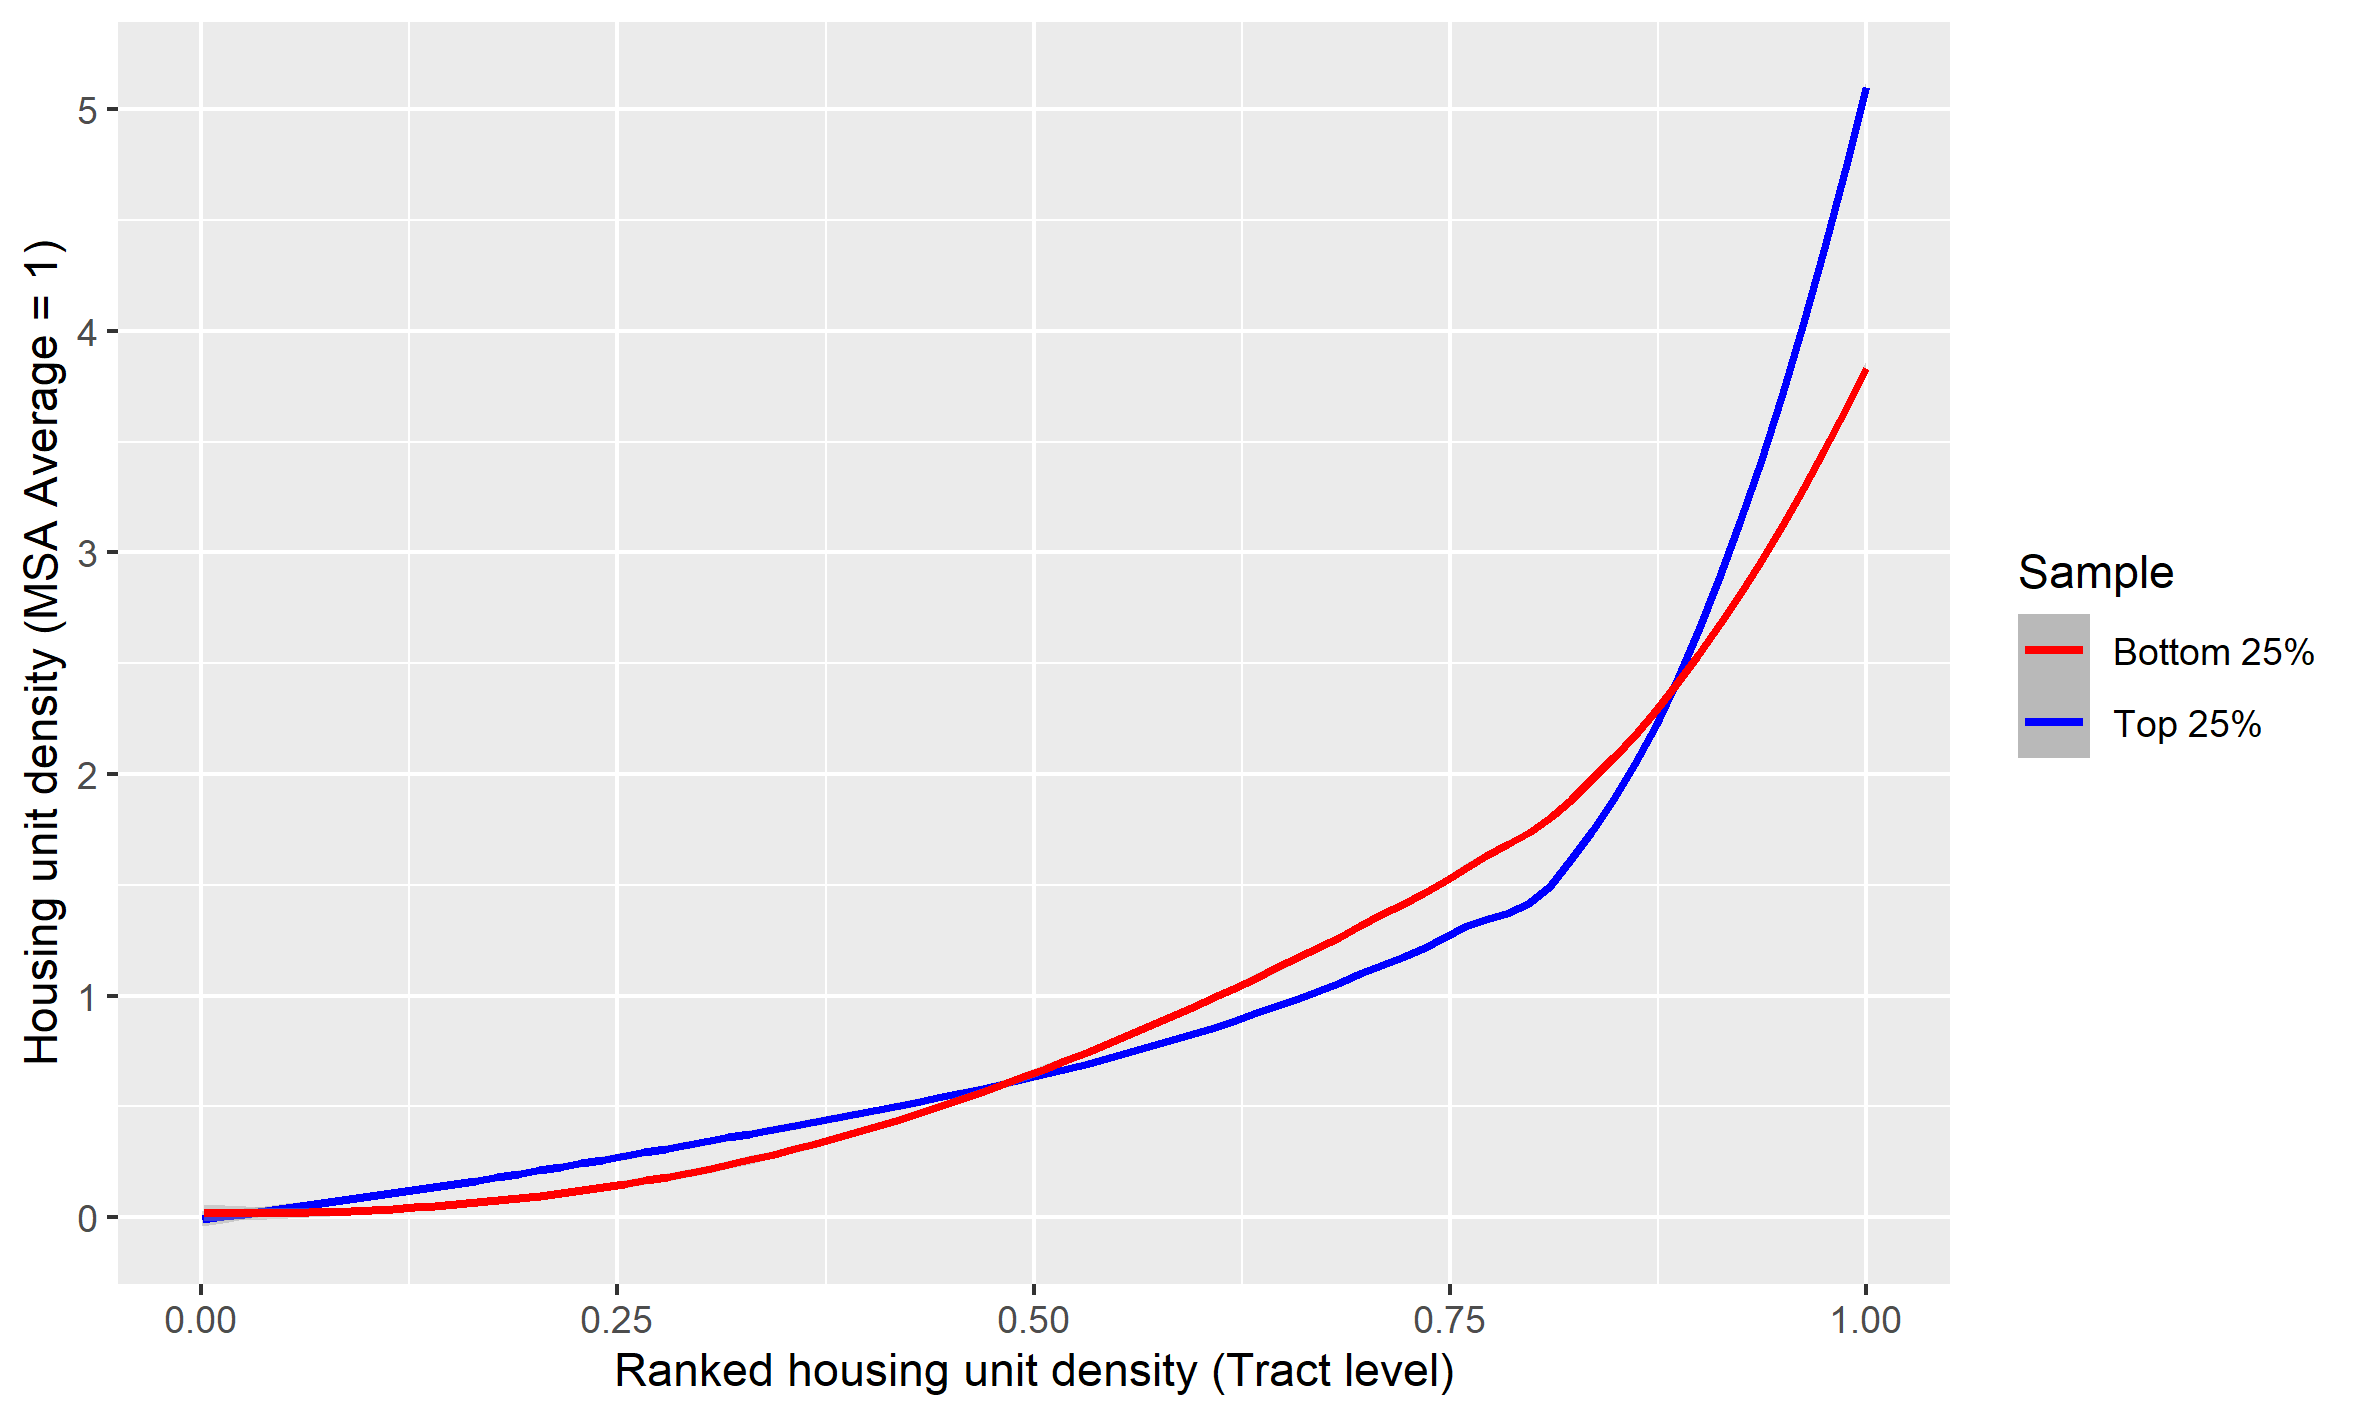
\includegraphics[width=\textwidth]{tractdens_dist}
		\caption{Loess regression of within MSA housing unit density ranks against actual values of housing unit density, with smoothing parameter $\alpha = 0.5$. The average of housing unit density is normalized to 1 in each MSA to control for fixed effects. Data are from the 2010 Census. 95 percent confidence intervals are reported, but tight enough to be hidden by the drawn regression line.}
		\label{tractdens_dist}
	\end{figure}
\end{center}

\begin{figure}[htbp!]
	\vspace{-2cm}
	\centerline{	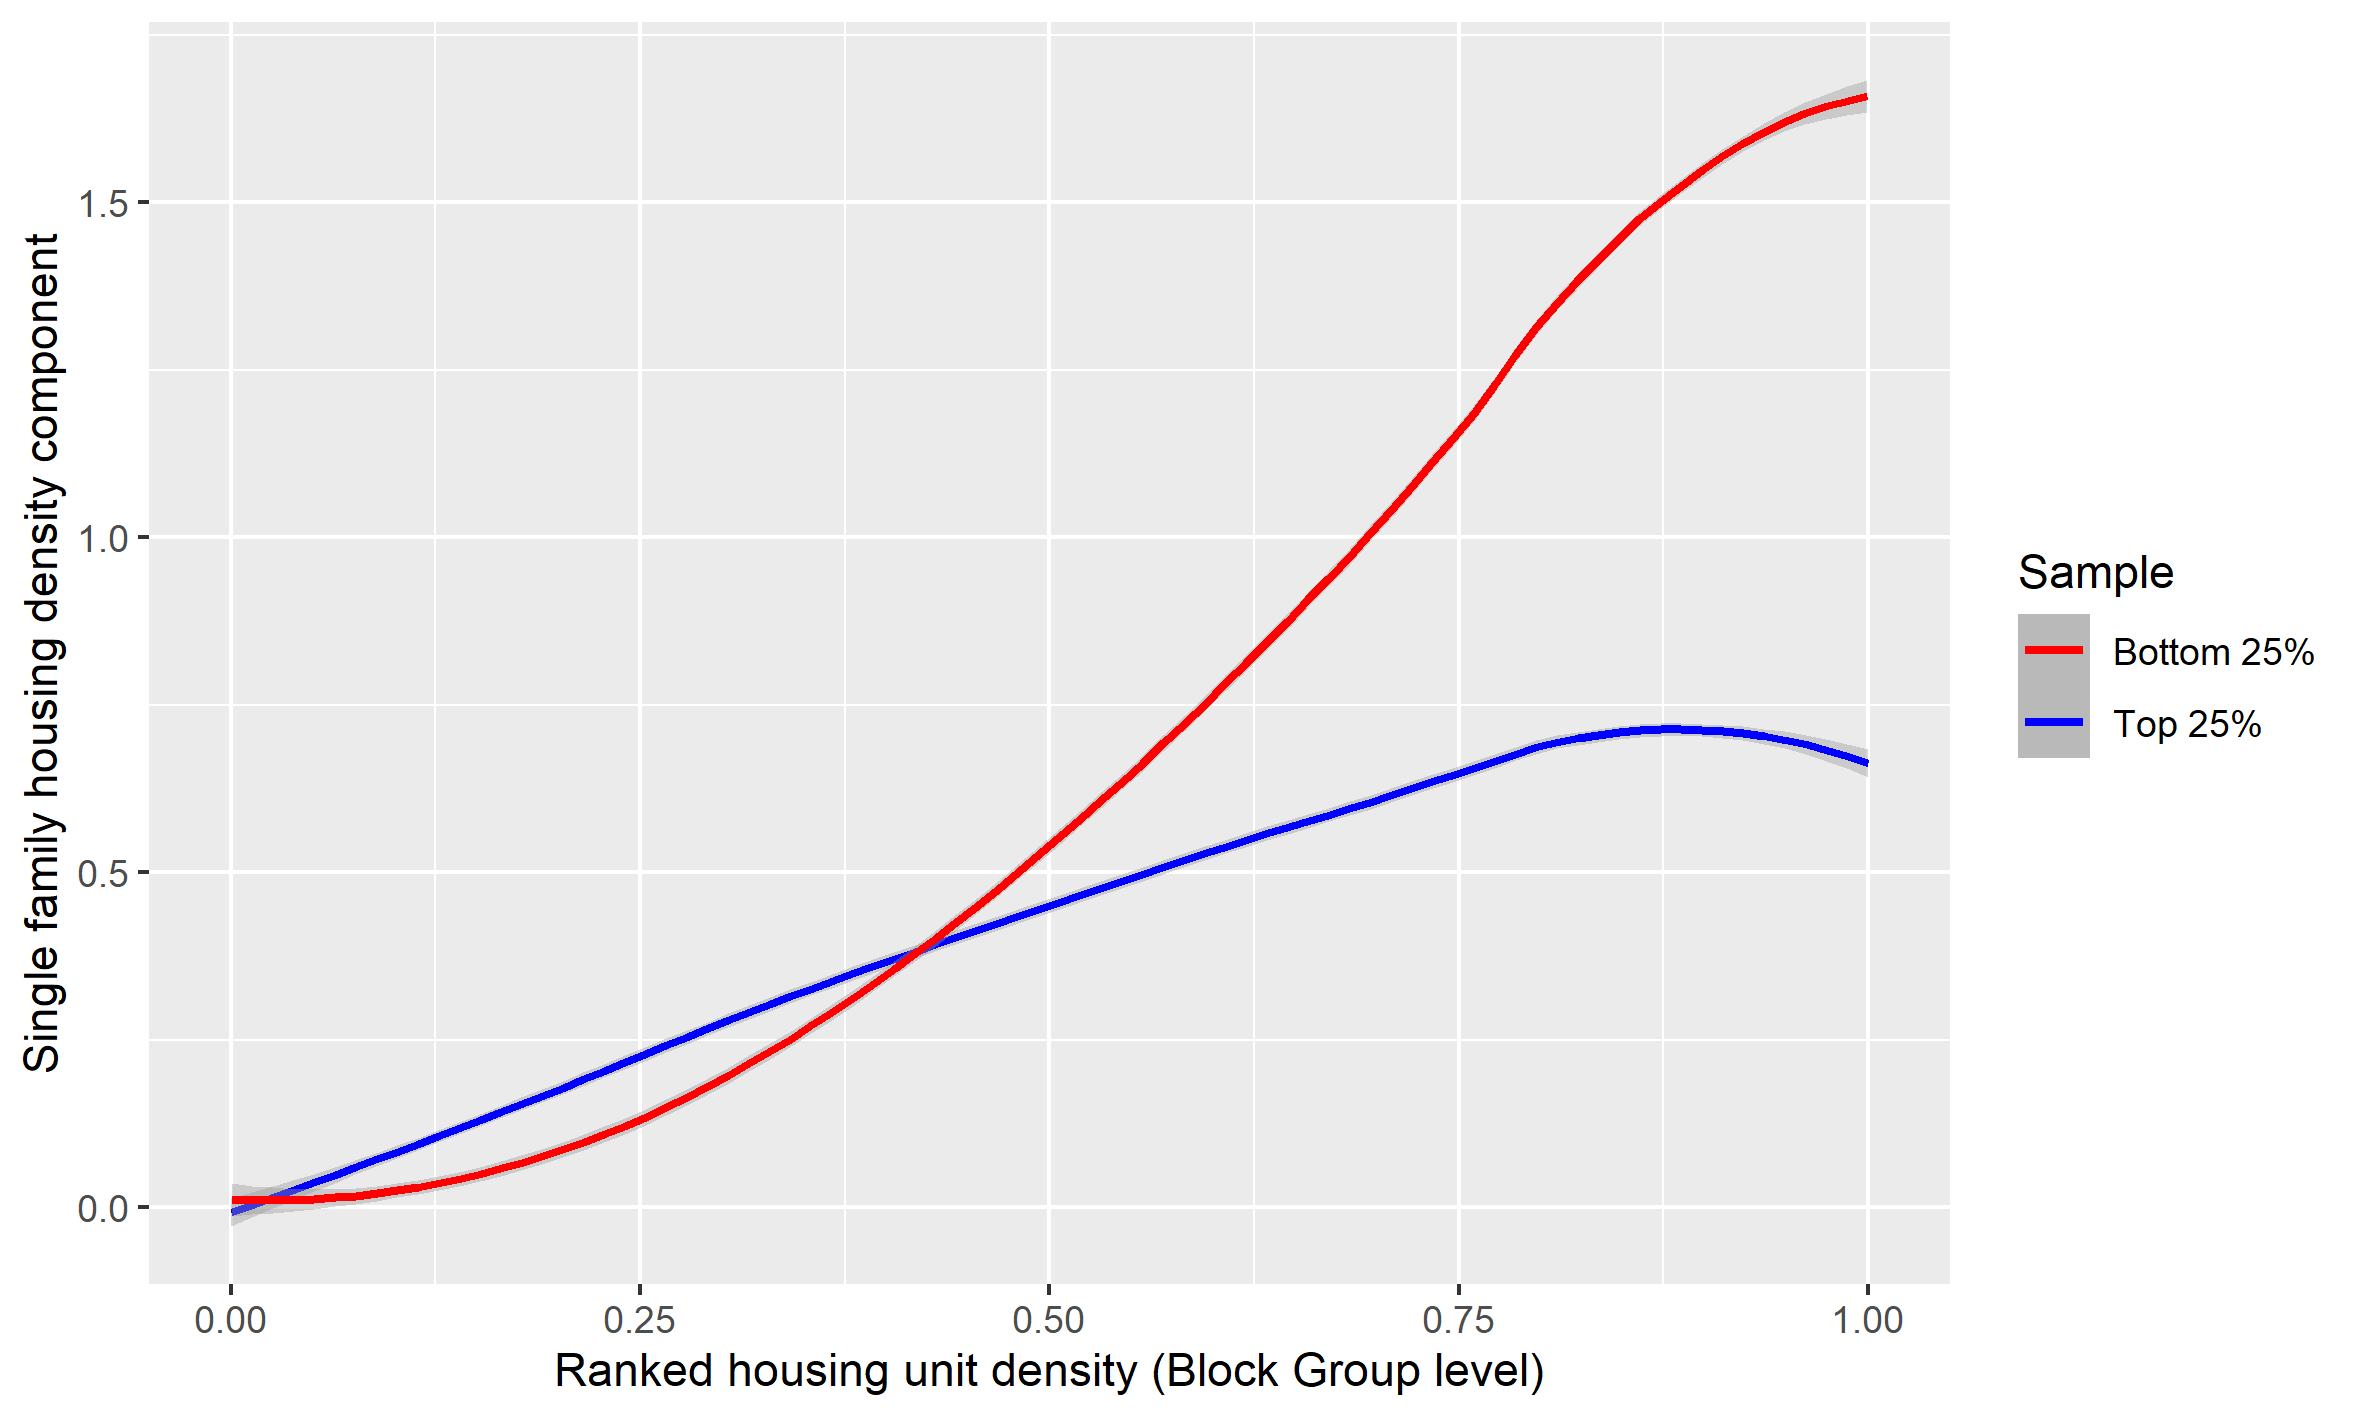
\includegraphics[width=\textwidth]{singlefamily_dist.png}}
	\centerline{	
	\includegraphics[width=\textwidth]{219building_dist.png}}
	\centerline{	
	\includegraphics[width=\textwidth]{20building_dist.png}}
		\caption{Loess regression of within MSA housing unit density ranks against each component of housing unit density, with smoothing parameter $\alpha = 0.5$. See Equation \eqref{Unit_decomp} for details. The average of housing unit density is normalized to 1 in each MSA to control for fixed effects. Total housing counts are from the 2010 Census, and shares of housing units in different structure types are from the 2008-2012 ACS. 95 percent confidence intervals are reported, but tight enough to be hidden by the drawn regression line for most of the range of the data.}
		\label{tractdens_decomp}
	\end{figure}		
\newpage

\begin{center}
	\begin{figure}[htbp!]
		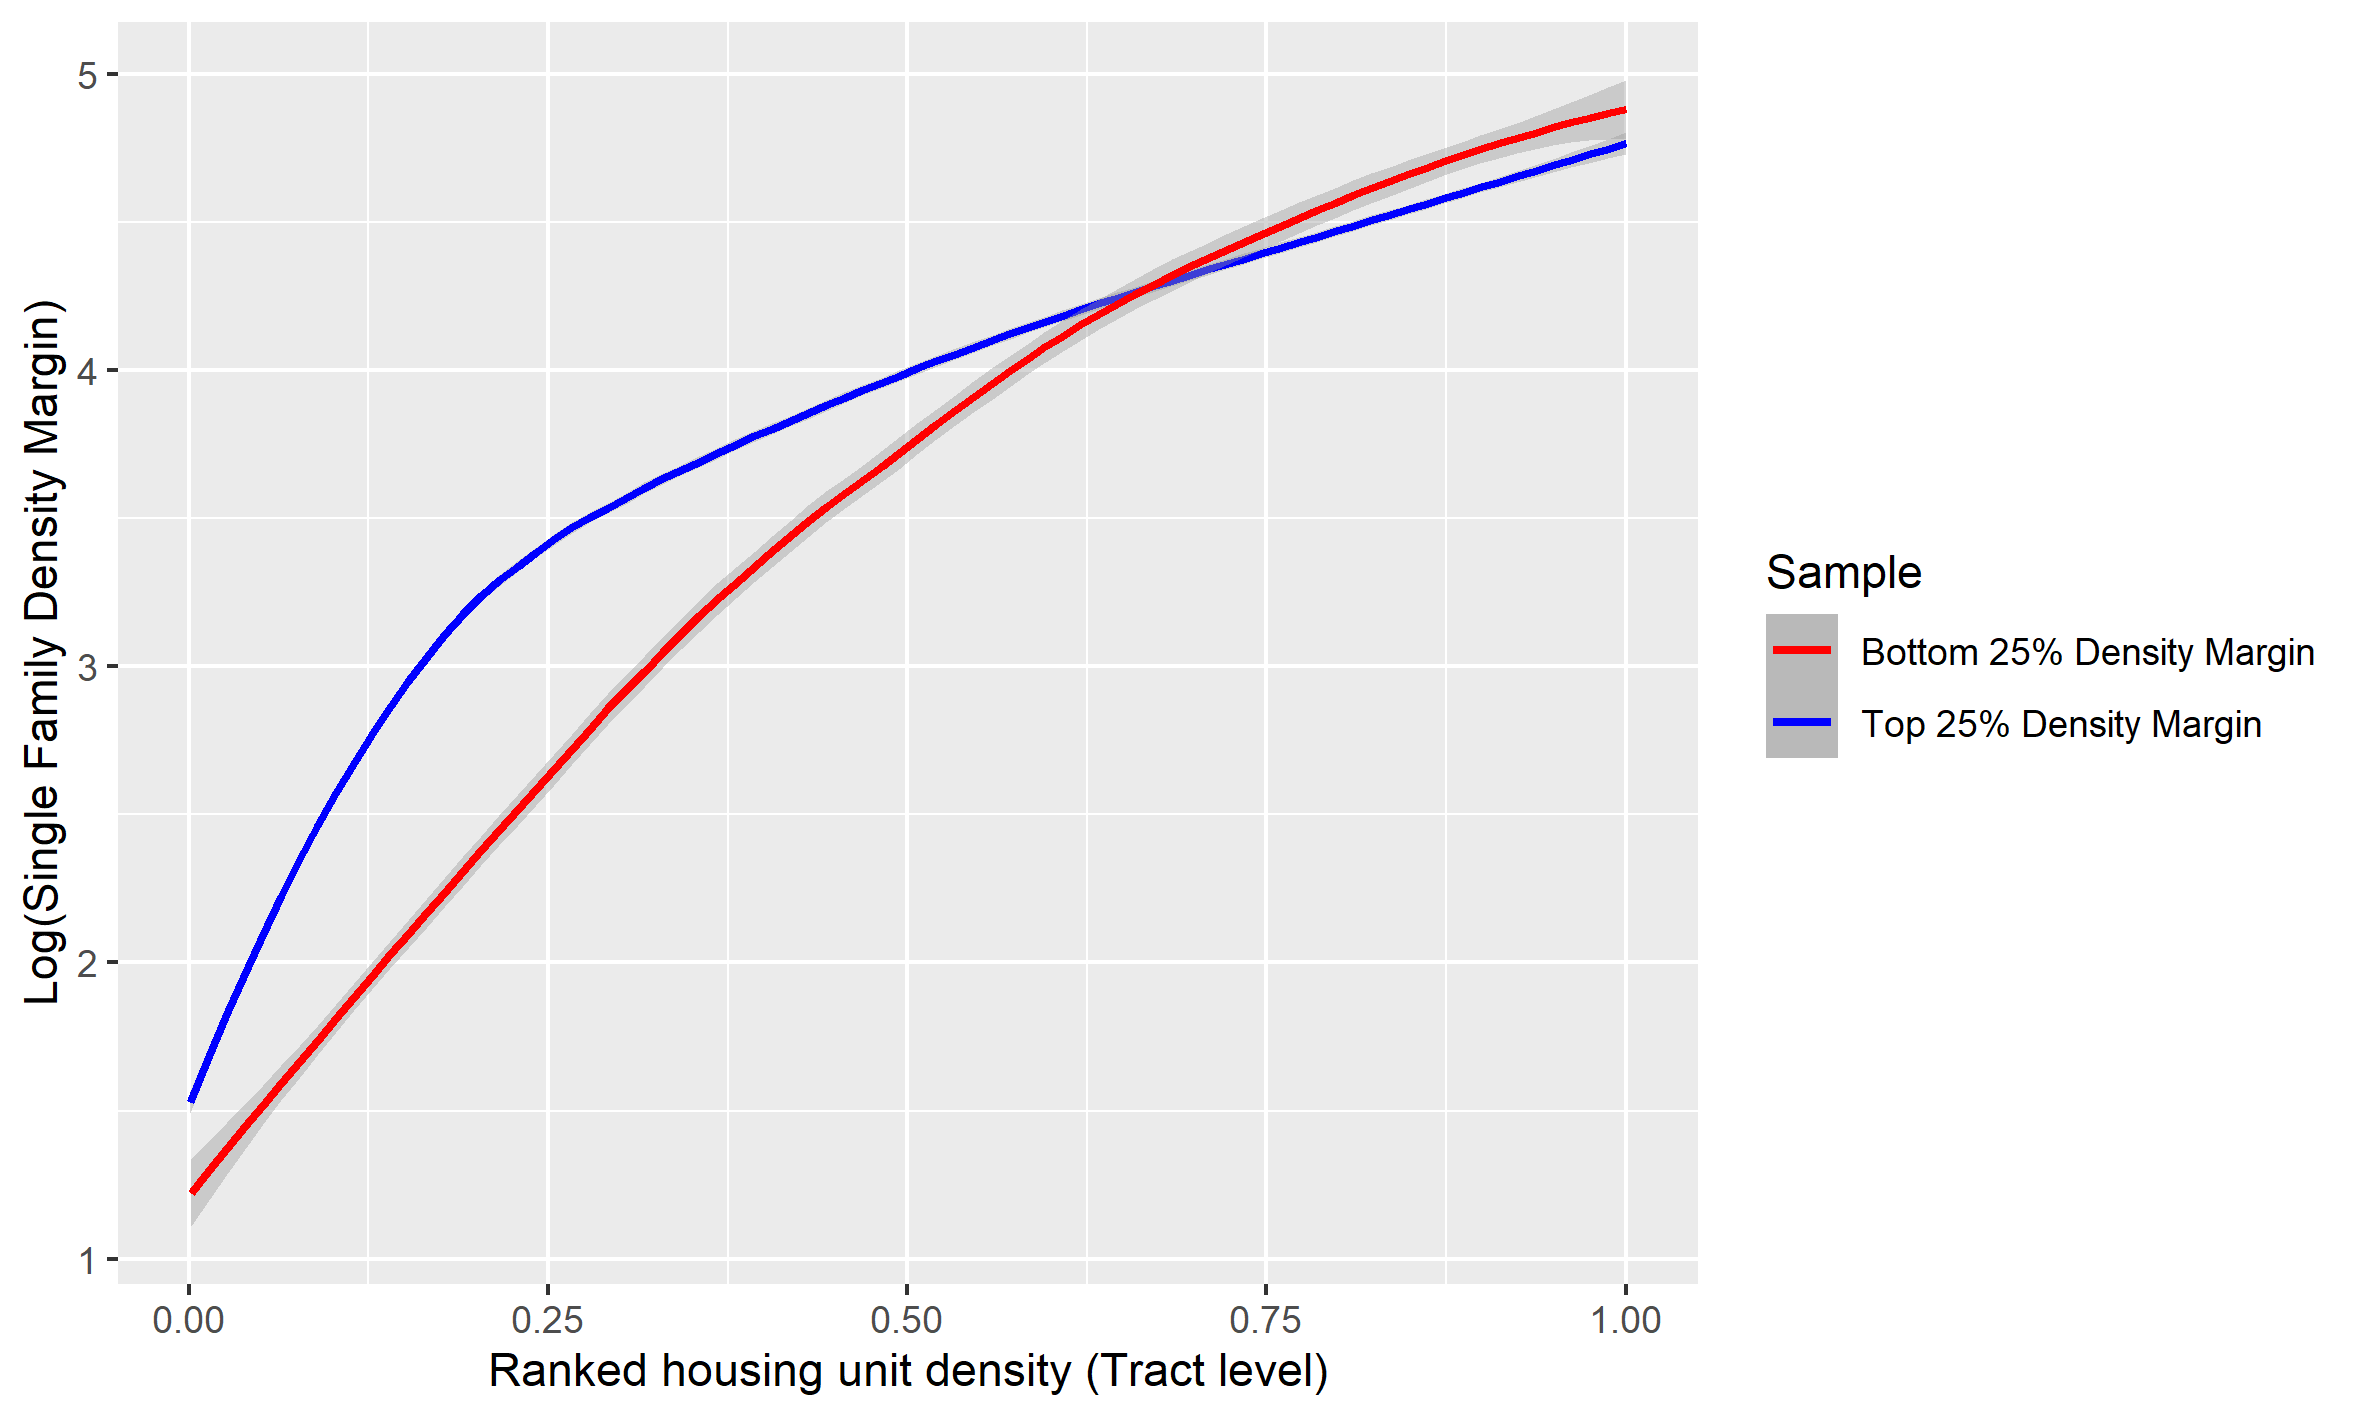
\includegraphics[width=\textwidth]{SingleFamilyDensity.png}
		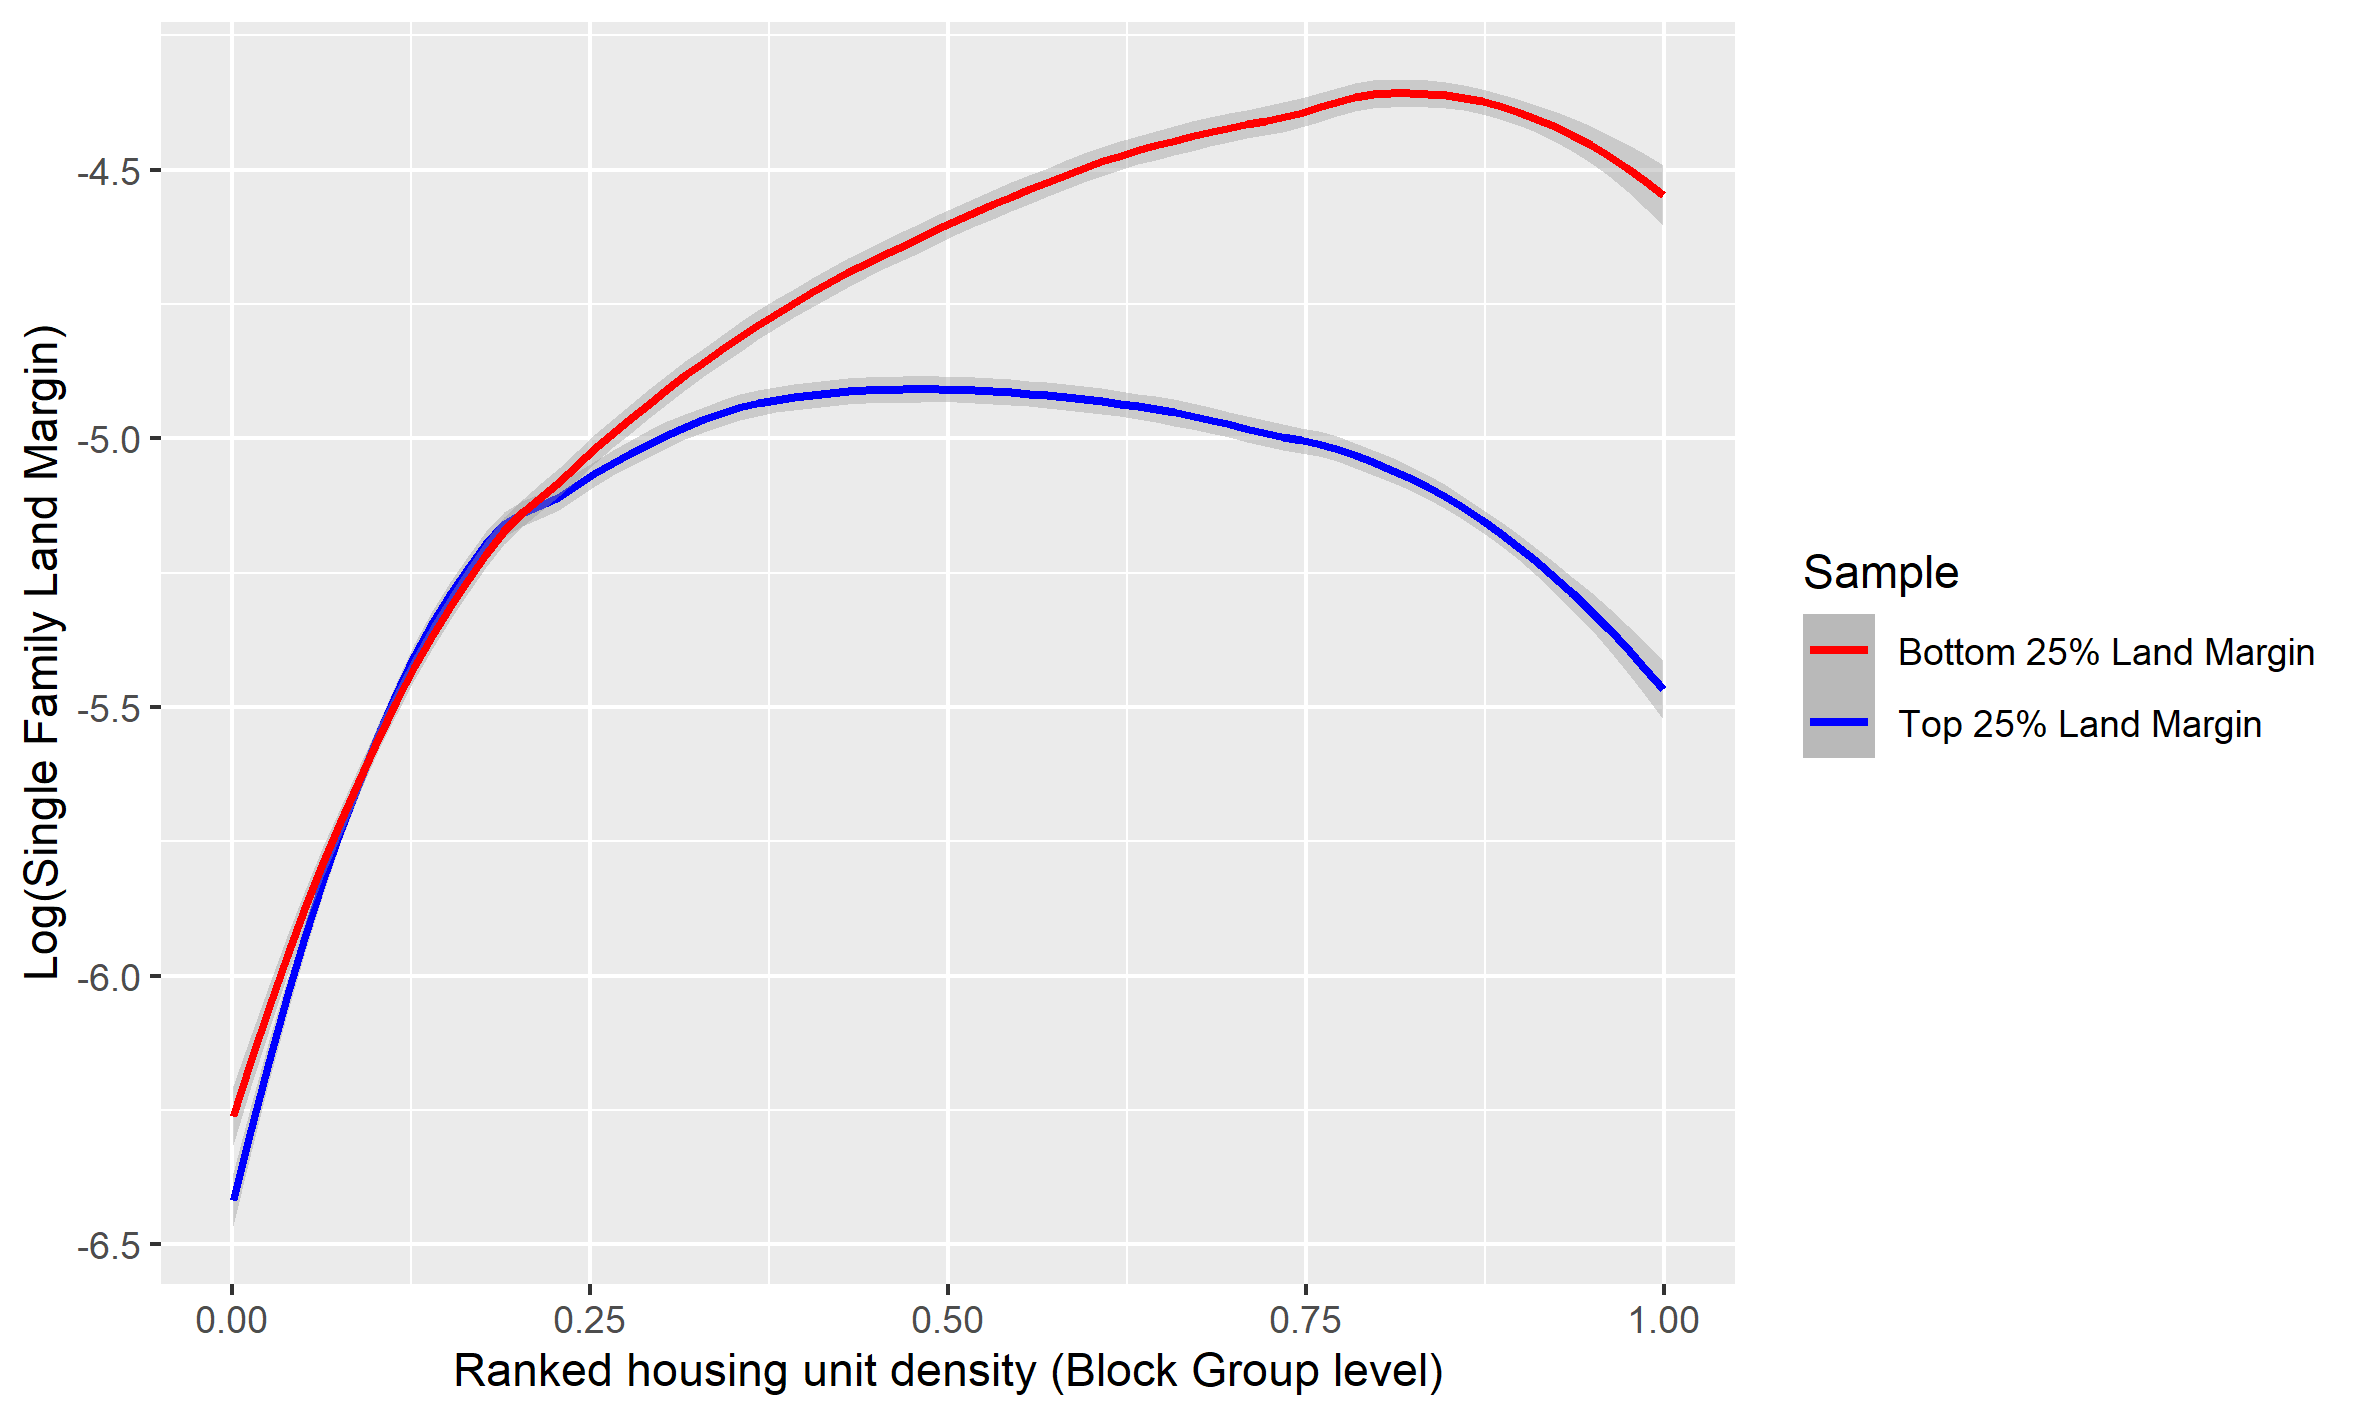
\includegraphics[width=\textwidth]{SingleFamilyLand.png}
		\caption{Loess regression of within MSA housing unit density ranks against the \textit{land} and \textit{density} margins of single family housing with smoothing parameter $\alpha = 0.5$. See Equation \eqref{SFdensdecomp} for details. The average of housing unit density is normalized to 1 in each MSA to control for fixed effects. Total housing counts are from the 2010 Census, and shares of housing units in different structure types are from the 2008-2012 ACS. 95 percent confidence intervals are reported, but tight enough to be hidden by the drawn regression line for most of the range of the data, depending on the regression.}
		\label{SFlanddensity}
	\end{figure}
\end{center}


\begin{center}
	\begin{figure}[htbp!]
	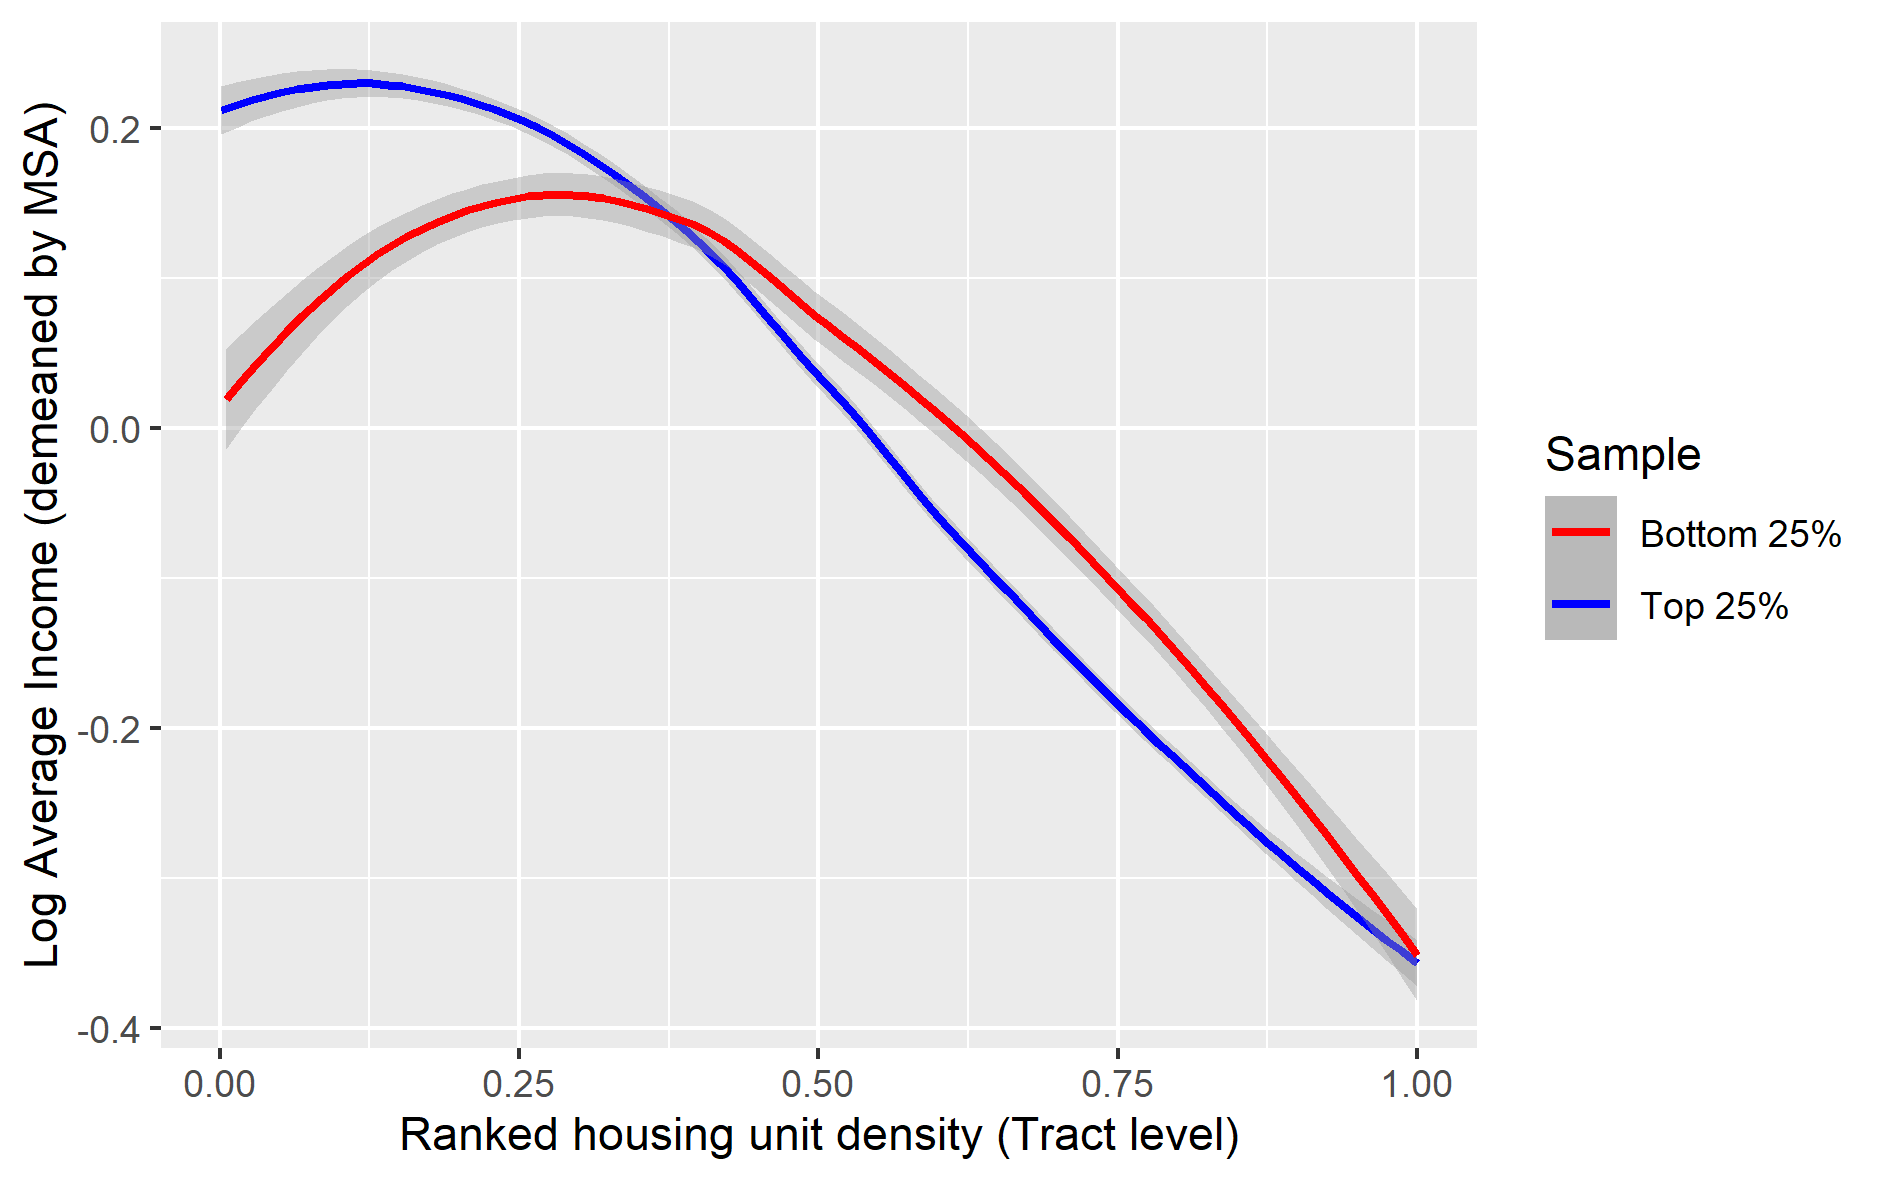
\includegraphics[width=\textwidth]{income.png}
	\caption{Average income is from the 2008-2012 ACS sample. Loess regression parameter $\alpha = 0.5$.}
	\label{income}
	\end{figure}
\end{center}

%
%\begin{center}
%	\begin{figure}[htbp!]
%		\includegraphics[width=\textwidth]{supplyelasticity.png}
%		\caption{hi}
%		\label{supplyelasticity}
%	\end{figure}
%\end{center}

\end{document}
